\section{Cytologie}

\subsection{Basics}

\begin{itemize}
	\item Domänen: Bacteria, Archaea und Eukarya
	\item Verhältnis Oberfläche/Volumen 
	\item Gramfärbung benötigt Kristallviolett (g+) und Safranin (g-),
		zwischendurch Entfärbung von Kristallviolett mit Ethanol.
		Ethanol verschließt Peptidoglycanschicht von Grampositiven,
		deshalb wird die Farbe nicht entzogen.
	\item Haupttypen der Morphologie: 
		Kokken,
		Stäbchen,
		Spirillen,
		Spirochäten,
		Knospende Bakterien,
		Bakterien mit Zennanhängen
		und filamentöse Bakterien
\end{itemize}

\begin{description}
	\item[gram-positiv]
		Eigenschaft einer prokaryotischen Zelle,
		deren Zellwand vorallem aus Peptidoglycan besteht
		und der die äußere Membran von gram-negativen Zellen fehlt.

	\item[gram-negativ] 
		Eigenschaft einer prokrayotischen zelle,
		deren Zellwand geringe Mengen von Petidoglycan enthält.
		Sowie eine äußere Membran,
		die Lipopolysaccahride,
		Lipoproteine,
		und andere komplexe Makromoleküle enthält.

	\item[Peptidoglycan]
		Polysaccharid,
		das aus alternierenden Wiederholungen von Acetyglucosamin und Actylmuraminsäuren besteht,
		die in benachbarten Shichten angeordnet
		und durch kurze Peptide quervernetzt sind.

\end{description}

In Tabelle \ref{tab:domaenenuberblick} ist eine Übersich über die Eigenschaften der drei Organismenreiche.	

\begin{table}[h!]
	\begin{center}
		\begin{tabular}{l l l l} 
			\toprule
			Merkmal		&	Bacteria		&	 Archaea				&	 Eukaraya		\\
			\midrule
			Zellkern 	&	nein			&	 nein					&	 ja		\\
			cccDNA		&	ja				&	 ja					&	 nein (linear)			\\
			Histone		&	nein			&	 ja					&	 ja		\\
			Zellwand		&	Murein		&	 kein Murein		&	 kein Murein		\\
			Membranlipid&	Ester			&	 Ether				&	 Ester		\\
			\midrule
			Ribosomen	&	70S			&	 70S					&	 80S		\\
			Ini-tRNA		&	f-Met			&	 Met					&	 Met		\\
			Introns 		&	nein			&	 nein					&	 ja		\\
			ja				&	Operon		&	 ns					&	 nein		\\
			Cap/poly-A 	&	nein			&	 nein					&	 ja		\\
			Plasmide		&	ja				&	 ja					&	 selten		\\
			RNA-Pol			&	ne (4 UE)	&	 viele (8-12 UE)	&	drei (12-14 UE)	\\
			TK-Faktoren		&	nicht nötig	&	 benötigt			&	benötigt		\\
			Promotoren		&	-10, -35		&	 TATA					&	TATA		\\
			\midrule
			Methanbildung		&	nein			&	 ja					&	nein		\\
			S-Reduktion		&	ja				&	 ja					&	nein		\\
			Nitrifizierung	&	ja				&	 nein					&	nein		\\
			Denitrifizierung		&	ja				&	 ja					&	nein		\\
			N-Fixierung		&	ja				&	 ja					&	nein		\\
			Photosynthese		&	ja				&	 nein					&	nein (Plastiden)	\\
			Lithotrophie	&	ja				&	 ja					&	nein		\\
			Grw. > 80°C		&	ja				&	 ja					&	nein		\\
			\bottomrule
		\end{tabular}
		\caption{Übersicht über die Eigenschaften der drei Organismenreiche.}
		\label{tab:domaenenuberblick}
	\end{center}
\end{table}

\subsection{Aufbau}

\subsubsection{Eukarya}
\begin{figure}[ht!]
	\leavevmode
	\begin{center}
		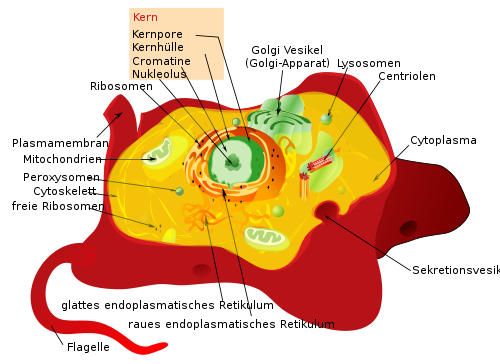
\includegraphics[scale=0.47]{./pictures/animal_cell_500}
	\end{center}
	\caption{\slshape{Tierische Zelle als Beispiel einer eukaryotischen Zelle.}}
	\label{fig:eukarya}
\end{figure}

\subsubsection{Prokarya}
\begin{figure}[ht!]
	\leavevmode
	\begin{center}
		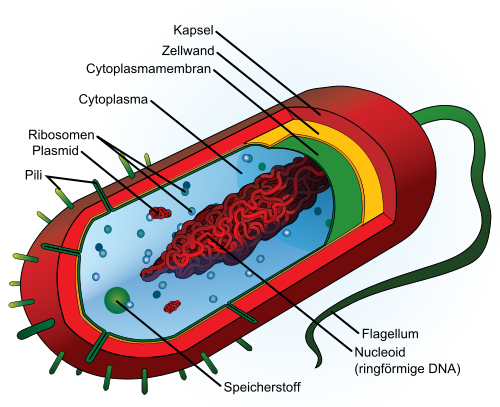
\includegraphics[scale=0.47]{./pictures/avg_prokaryote_cell_500}
	\end{center}
	\caption{\slshape{Typische prokaryotische Zelle.}}
	\label{fig:prokarya}
\end{figure}

\subsubsection{Endosporen}

\begin{itemize}
	\item Überdauerungstadium
	\item steigert Resistenz gegen schädliche äußere Einflüsse
	\item kein/kaum Metabolismus
	\item Reduktion des Wassergehaltes auf 10-25\% im Kern
	\item meist von gram-positive Zellen, auch einige gram-negative
\end{itemize}

\subsubsection{Bewegung mit Geißeln}

\begin{description}
	\item[Aufbau] \hfill \\
		Der typische Aufbau ist in Abbildung \ref{fig:flagellum},
		für ein Gram-negatives Bakterium dargestellt.

		Das Flagellum selbst besteht aus Untereinheiten des Moleküls Flagllin.
		Der Haken ist aus einem einzigen Protein und verbindet den ``Motor'' mit dem Filament.

		Der Motor ist mit Rotor und Stator in die Zellwand eingelassen,
		wobei er alle Schichten durchdringt.
		Der Stator ist Bestandteil der Cytoplasmamembran.
		
		Bestandteile des Rotos sind:
		\begin{description}
			\item[L-Ring] Lipopolysaccharidschicht
			\item[P-Ring] Petidoglycanschicht
			\item[MS-Ring \& C-Ring] Cytoplasmamembran und Cytoplasma
		\end{description}

		Zwischen MS- und C-Ring befinden sich Fli-Proteine,
		welche mit dem Mot-Protein die Bewegung vermitteln.

		\begin{figure}[ht!]
			\leavevmode
			\begin{center}
				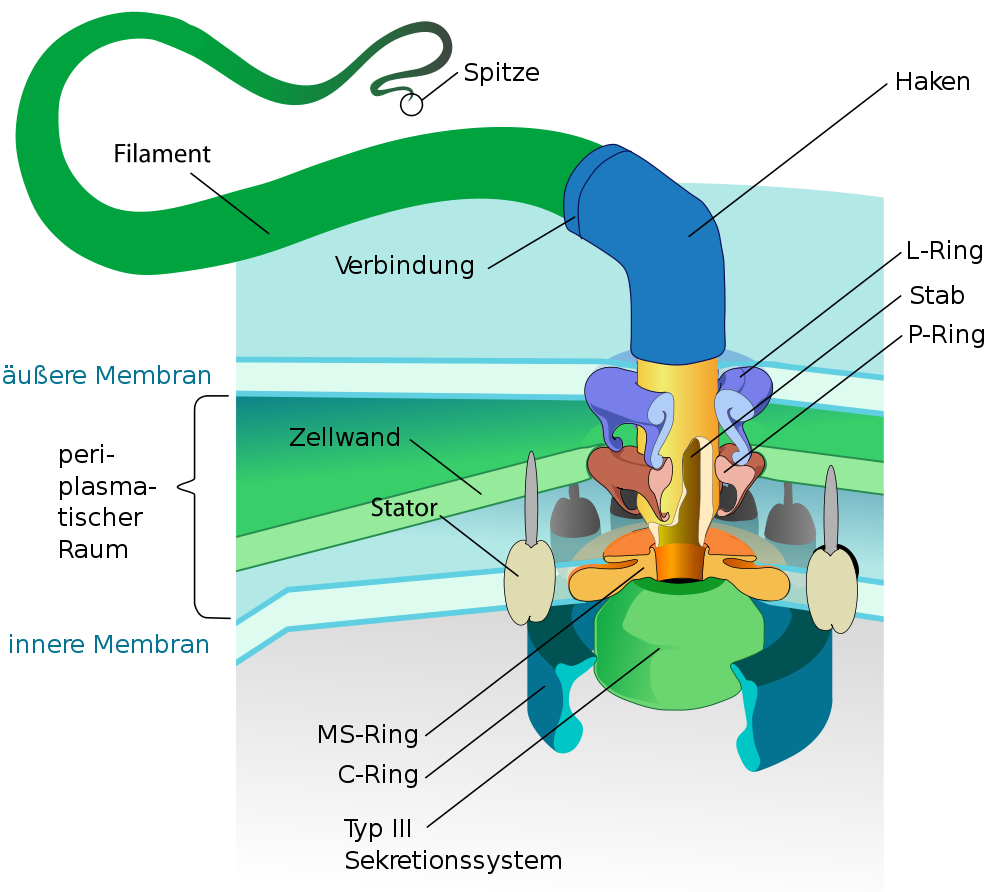
\includegraphics[scale=0.3]{./pictures/flagellum_1k}
			\end{center}
			\caption{\slshape{Motorkomplex eines Gram-negativen Bakteriums.}}
			% http://de.wikipedia.org/w/index.php?title=Datei:Flagellum_base_diagram_de.svg&filetimestamp=20110817105413
			\label{fig:flagellum}
		\end{figure}

	\item[Ablauf der Bewegung] \hfill \\
		Getrieben duch die Protonenmotorische Kraft,
		strömen \ce{H+} durch das Mot-Protein.
		Durch die versetzte Anordnung von positiven und negativen Ladungen auf den Ringen,
		und den Durchstrom der positiven Ladung,
		wird eine Drehbewegung über die Ringe auf den Schaft des Flagllums übetragen.

		Die Geschwindigkeit kann bis zu 60 Körperlängen/Sekunde erreichen,
		ein Gepard erreicht nur 25 Körperlängen/Sekunde.

	\item[Synthese] \hfill \\
		Zunächst wird der MS-Ring synthetisiert und schiebt sich in die Cytoplasmamembran.
		Dann werden die Motorproteinen und die Ringe bis zum Hacken synthetisiert.
		Anschließend bildet sich eine Kappe am Ende Des Hackens.
		Zwischen hacken und der Kappe werden nun Flagelin Proteine eingebaut,
		welche durch einen Kanal vom Cytoplasma in Richtung Kappe fließen.

		Abgebrochene Filamente können so auch repariert werden.

	\item[Steuerung] \hfill \\
		Wiederhole:
		\begin{enumerate}
			\item gebündelte Geißeln zur Fortbewegung in eine Richtung
			\item zertstreute Geißeln zum Taumeln und Neu-Orientieren
			\item gebündelte Geißeln zur Fortbewegung in eine Richtung
		\end{enumerate}

	\item[Orientierung] \hfill \\
		\begin{description}
			\item[Phototaxis]
			\item[Chemotaxis]
		\end{description}

\end{description}

\subsection{Membran}
\begin{description}
	\item[Einheitsmembranen (unit membrane)] \hfill \\
		\begin{itemize}
			\item Doppelschicht aus amphiphilen Fettsäuren (8 nm)
			\item ungesättigte Fettsäuren führen zu erhöhter Fluidität
			\item Temperaturanpassung, fluider: Cholesterin (Eukarya)
			\item Temperaturanpassung, starrer: Sterole (Eukarya), Hopanoide (Prokarya), nicht in Archaea
			\item Archaea: Ether- statt Esther-Bindung zwischen Glycerin und hydrophoben Seitenketten; 
				Isopren-ketten statt Fettsäuren; Auch: Monolayer durch verknüpfte Lipide
			\item Funktion: Permeabilitätsbarriere, Proteinverankerung, Energiekonservierung
		\end{itemize}

	\item[Äußere Membran (outermembrane)] \hfill \\
		\begin{itemize}
			\item Peptidoglycanschicht
			\item Periplasma
		\end{itemize}

	\item[Transport] \hfill \\
		\begin{itemize}
			\item Einfacher Transport, getrieben durch protonenmotorische Kraft
			\item Gruppentranslokation, chemische Veränderung der transportierten Verbindung,
				getrieben durch Phophoenolpyruvat
			\item ABC-System, mit Permiplasmatischen Bindeproteinen,
				getrieben durch ATP
		\end{itemize}

	\item[Grampositive Zellwand] \hfill \\
		Cytoplasmamembran mit aufgelagerter Peptidoglycanschicht.
		Beide Schichten enthalten Membranproteine.
		Verbindung durch Lipoteichonsäuren,
		die durch die Peptidoglycanschicht bis in die Cytoplasmamembran reichen.
		Teichonsäuren reichen nur in die Peptidoglycanschicht.

		\begin{figure}[ht!]
			\leavevmode
			\begin{center}
				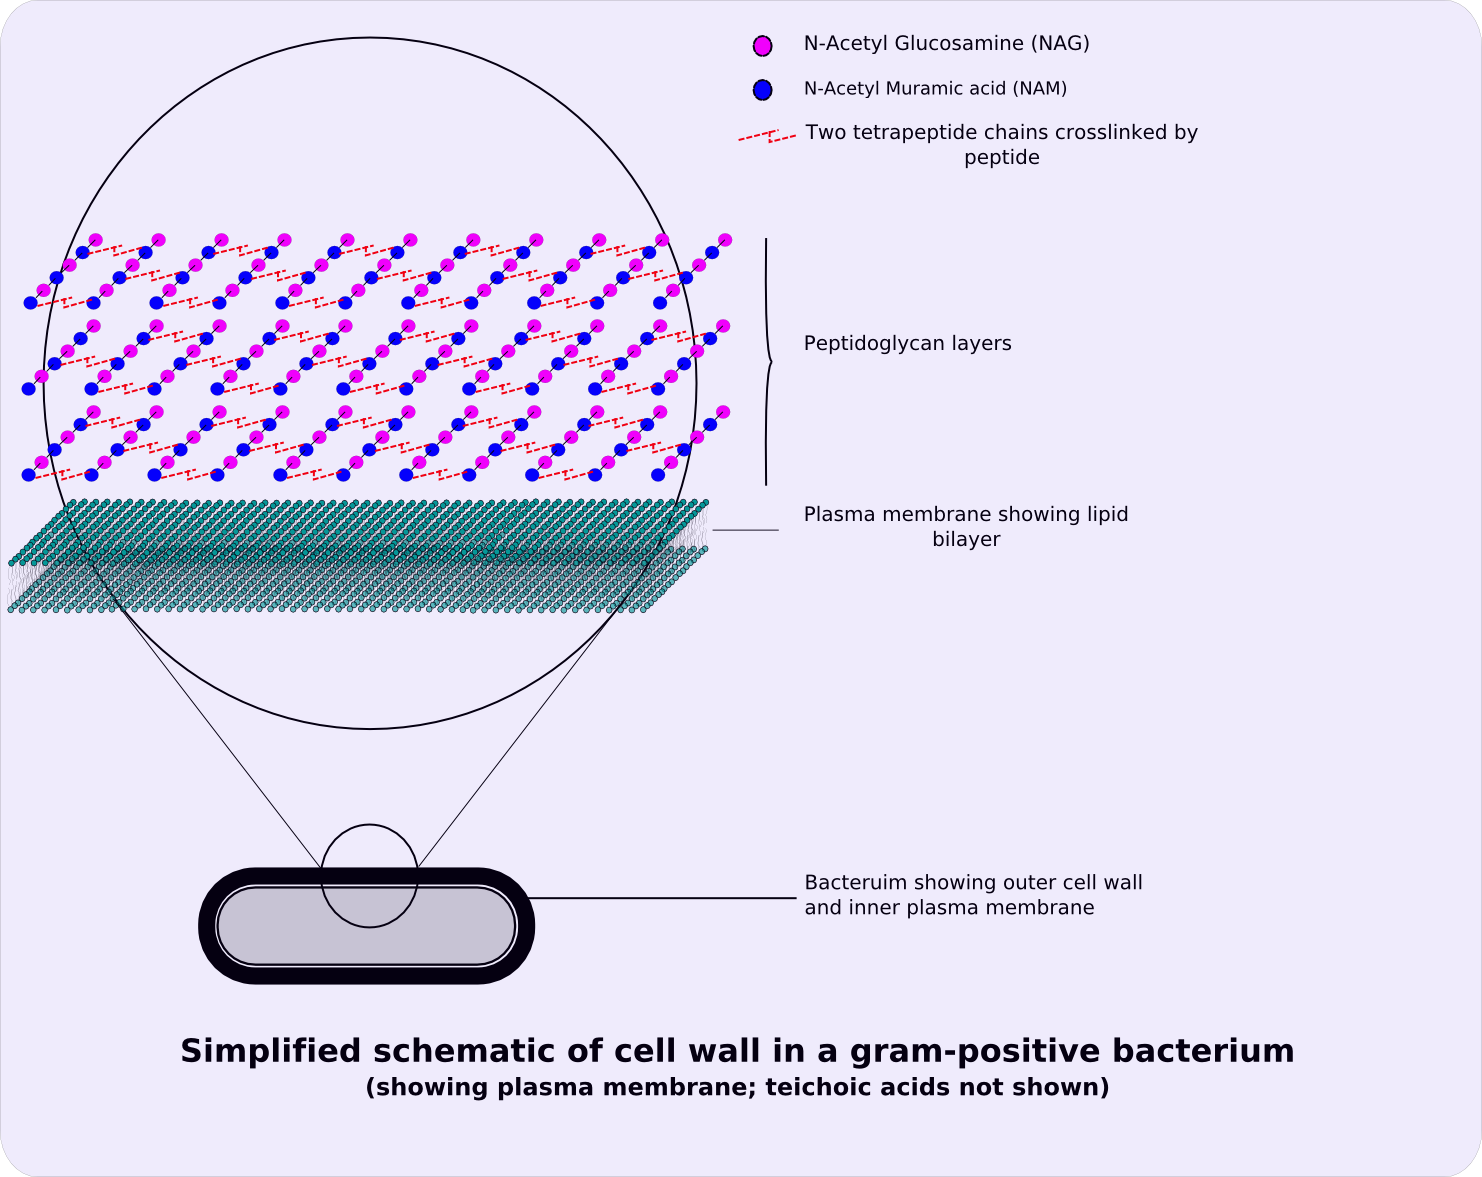
\includegraphics[scale=0.27]{./pictures/gram_positive_zw}
			\end{center}
			\caption{\slshape{Gram-Positive Zellwand der Bacteria.}}
			\label{fig:gramPosBacZW}
		\end{figure}

	\item[Gramnegative Zellwand] \hfill \\
		Zusätzlich zum Peptidoglycan eine Zusätzliche Äußere Membran.
		Sie ist aufgebaut wie die Cytoplasmamembran,
		enthält jedoch zusätzlich Polysaccharide,
		welche einen sogenannten Lipopolysaccharidkomplex bilden,
		daher auch Lipopolysaccharidschicht (LPS).

		Die Lipooplysaccharide sind dabei auf die äußere Membran aufgelagert
		und beinhaltet ebenfalls Transportproteine.
		Der Zwischenraum ober und unterhalb des Peptidoglycanschicht 
		wird als Periplasma bezeichnet.
		Die Verankerung der LPS erfolgt durch Lipoproteine mit der Peptidoglycanschicht.

		\begin{figure}[ht!]
			\leavevmode
			\begin{center}
				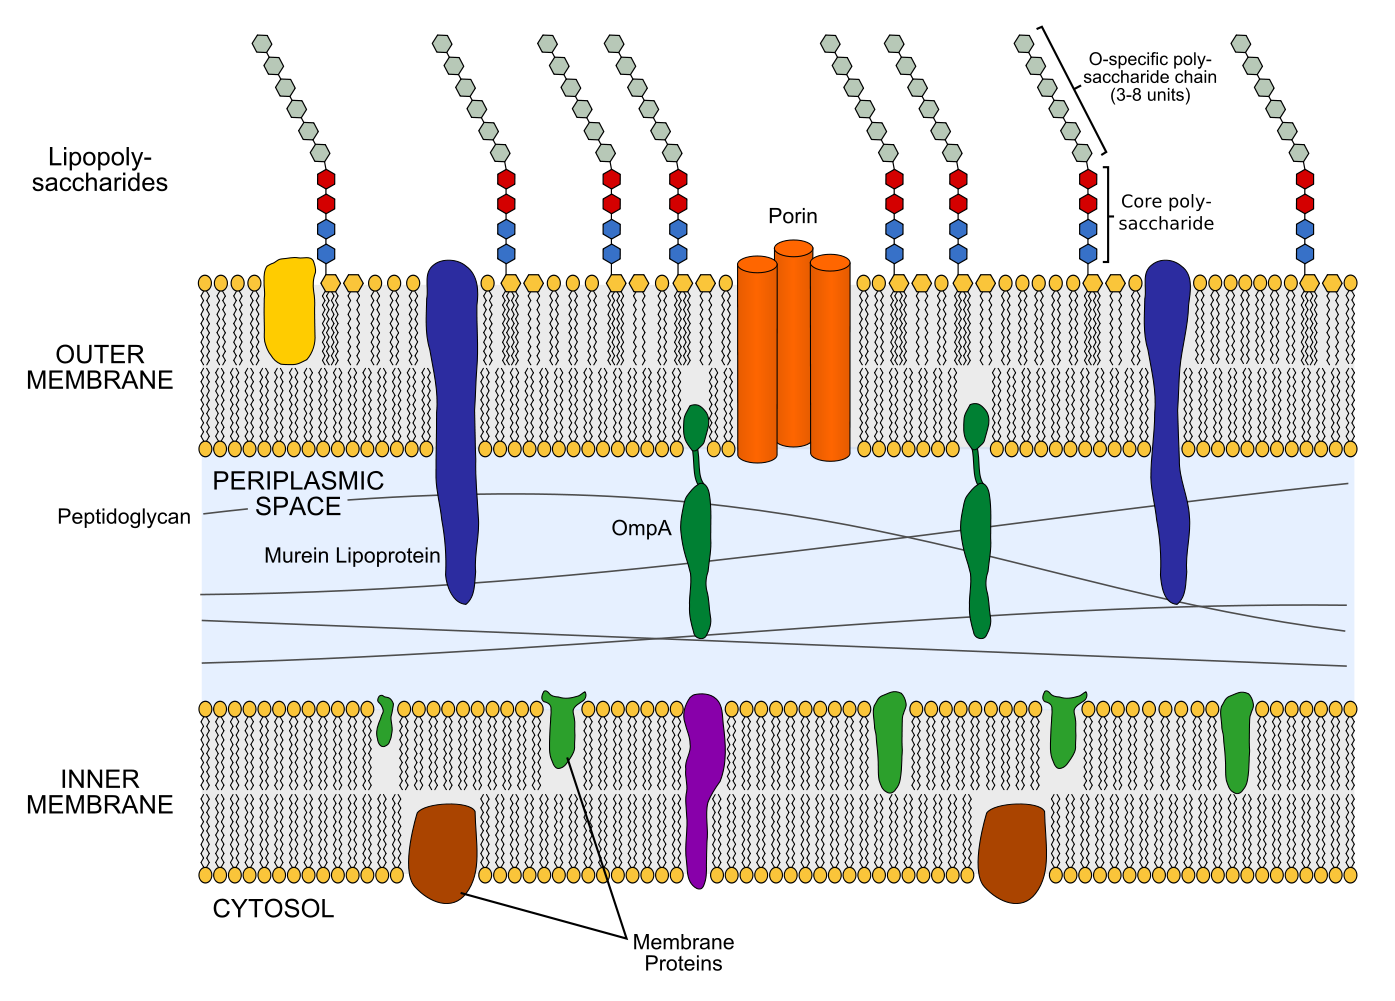
\includegraphics[scale=0.25]{./pictures/gram_negative_zw_noLegend}
			\end{center}
			\caption{\slshape{Gram-Negative Zellwand der Bacteria.}}
			\label{fig:gramNegBacZW}
		\end{figure}
\end{description}

\subsection{Zellwand}
